\subsection{Simulation framework}

The ATLAS simulation program is integrated into the ATLAS software framework called \textit{Athena}\cite{atlas:athena},
which uses Python as an object-oriented scripting and interpreter language to configure and load C++ algorithms and objects.
Figure~\ref{fig:frame_overview} shows the overview of ATLAS simulation data flow\cite{Aad:2010ah}.
In the diagrams, the square-cornered boxes represents algorithms and applications to be run and round-cornered boxes denote data objects.
\begin{figure}[!htb]
  \centering
  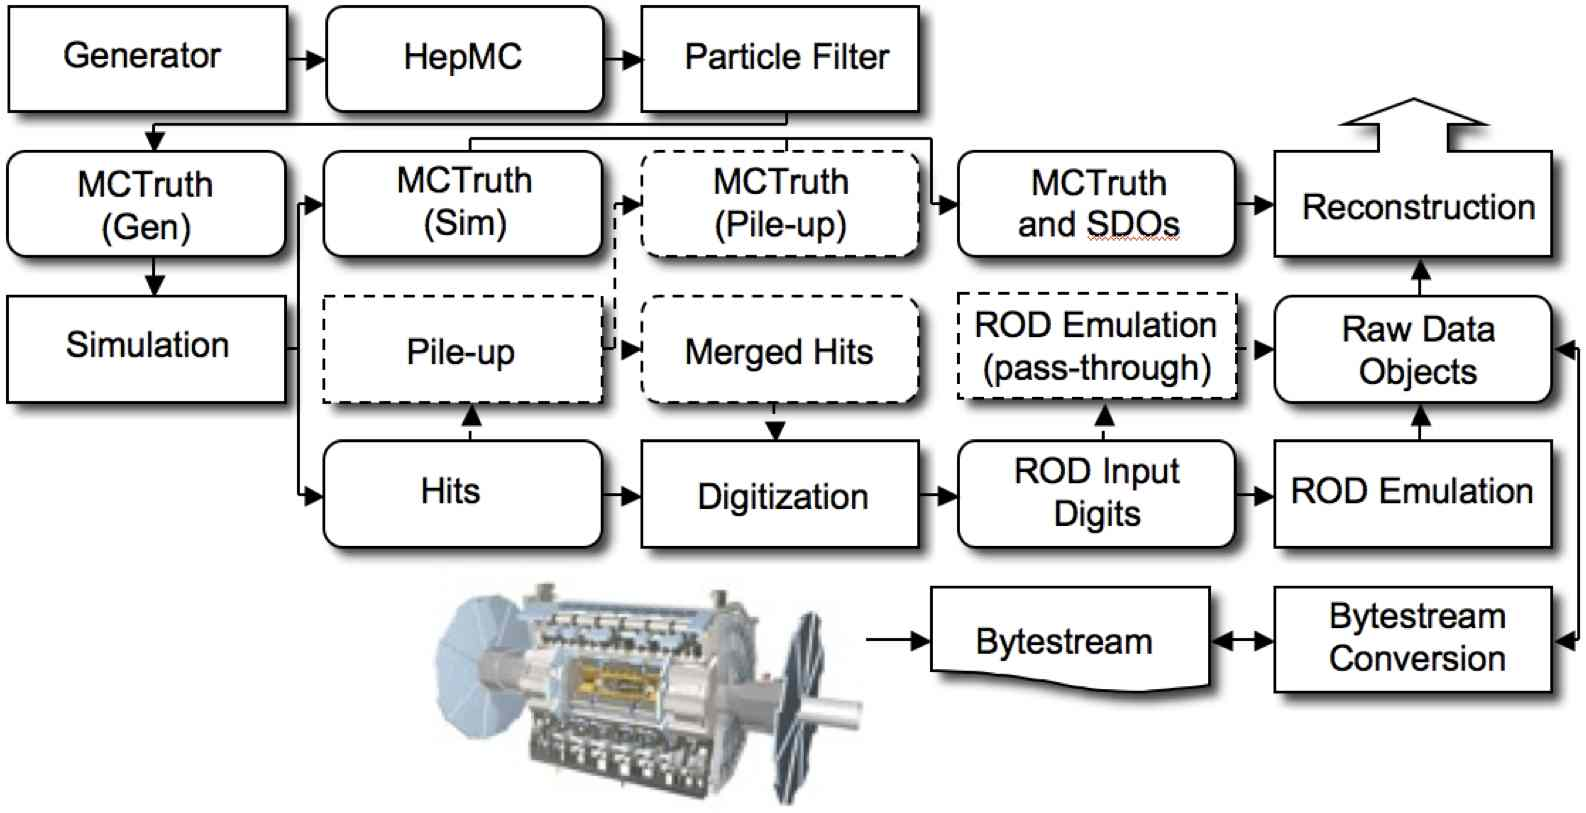
\includegraphics[width=1.0\textwidth]{figures/Simulation/outline_atalsSimulation_v2.png}
  \caption{The flow of the ATLAS simulation software.}
  \label{fig:frame_overview}
\end{figure}

First of all, events are produced by MC generators in standard HepMC format and then read into the simulation.
During the simulation, particles are propagated through the full ATLAS detector whose configurations can be set by users via GEANT4 toolkit.
The energies deposited in the sensitive regions of the detector are recorded as \textit{hits}, which contains the total energy deposition,
position, and time, and are written to a simulation hit file.
In the meatime, the events in "truth" format are also recorded to contain the history of the interactions from the generator, including incoming and outgoing particles.
Simulated Data Objects (SDOs) are created from truth, which are maps between hits in sensitive portions of the detector and truth information of particles in simulation.
The files are then sent to digitization, with constructs "digits" inputs and be written into Raw Data Object (RDO) file used for reconstruction.

In conclusion, there are three main parts of framework: \textit{Generation}, \textit{Simulation} and \textit{Digitization}.
More details are given below.

\textbf{Event generation}

As shown in figure~\ref{fig:mc_event_structure}\cite{Hoche:2014rga}, at hardon colliders, multiple scattering and rescattering effects arise, which must be simulated by Monte Carlo (MC) event generators to reflect the full complexity of those event structures.
Several MC event generators can be used to generate events originally in HepMC format.
The events can be filtered at generation time with some certain requirements (eg. decay channel or missing energy above a certain threshold).
The generator is responsible for any prompt decays (e.g. W or Z bosons) but stores any "stable" particle expected to propagate through a part of the detector. 
During the generation steps, any interactions with detector are ignored and only immediate decays are considered.

There are several MC generators that have been widely-used with general purpose, which include Sherpa\cite{Gleisberg_2009}, Herwig++\cite{Bahr2008}, PowhegBox\cite{Nason:2004rx}, MC@NLO\cite{Frixione_2002} and Pythia8\cite{Sjostrand:2007gs}.

\begin{figure}[!htb]
  \centering
  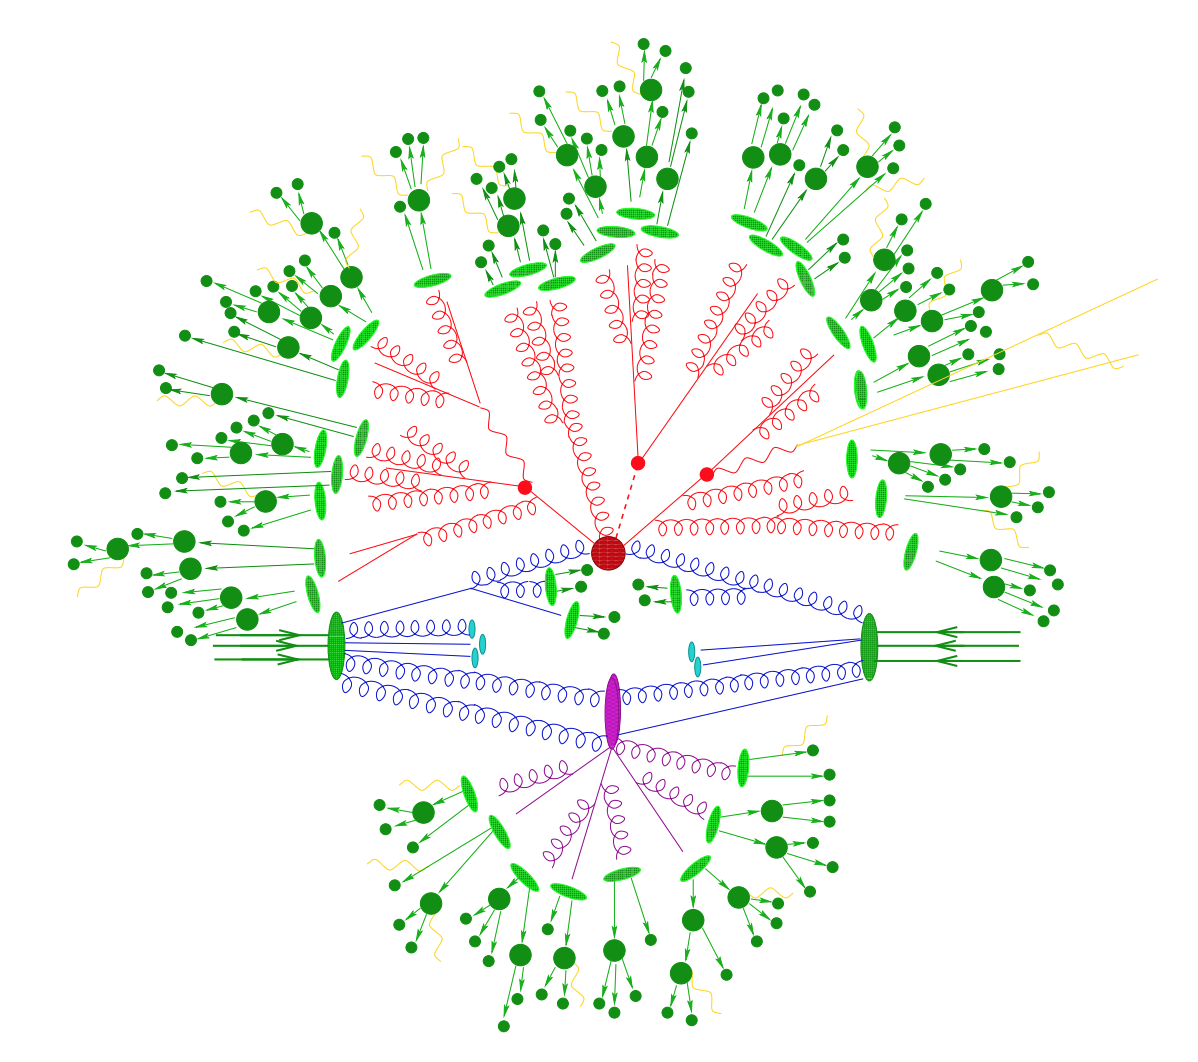
\includegraphics[width=0.7\textwidth]{figures/Simulation/mc_event_structure.png}
  \caption{Sketch of a hardon-hardon collision simulated by MC event generator. The red blob in center denotes the hard collision, surrounded by tree-like structures representing Bremsstrahlung which is simulated by Parton Showers. The purple blob stands for a secondary hard scattering event. The light green blobs indecate the parton-to-hardon transitions and the dark green blobs represents hardon decays. The yellow lines are soft photon radiations.}
  \label{fig:mc_event_structure}
\end{figure}

\textbf{Simulation}

GEANT4 is used as standard simulation toolkit for the ATLAS experiment, which transports physics particles through the detector's geometry.
During the generation level, the entire connected chain of the HepMC event is stored as the Monte Carlo truth. 
Only the stable particles are read into GEANT4 for further simulation and cuts and transformations can be applied to these events to select certain processes.
During the simulation, many secondary tracks can be produced, therefore only information from the interactions of interest are stored, including the incoming particles, step sequence, vertex and also outgoing particles.
The output of GEANT4 is called \textit{hit file}, which contains metadata describing the configuration of the simulation during the run, all truth information requested and a collection of hits for each subdetector.

Since the standard ATLAS detector simulation cost very large computing resources to accurately model the complex detector geometry and physics descriptions, some fast simulation programss are developed according to different user purpose.
Some widely-used fast-sim toolkits include \textit{Fast G4 Simulation}\cite{Barberio:2007gba}, \textit{ATLFAST-I}\cite{Richter-Was:683751} and \textit{ATLFAST-II}\cite{Edmonds:1091969}.

\textbf{Digitization}

The hit outputs from simulated events, including hard scattering signal, minimum bias, beam halo, beam gas and cavern background events, are then send into digitization to convert into detector response called "digits".
Before converting into detector signal with 'digits' formart, each type of events can be overlaid at a user-specified rate.
Those overlay, called "pile-up", can be done during degitization to save the CPU time in simulation level.
At this stage, the detector noise and the first level trigger that implemented with hardware on the real detector are added into events.
The digitization firstly constructs "digits" inputs to the read out drivers (RODs) in the detector electronics.
The ROD functionality is then emulated, and the output digits are written out as Raw Data Object (RDO) file.
In addition, the digitization algorithms can also produce Simulated Data Objects (SDOs), which contain information about all the particles, noise and the amount of energy that contributed to the signal. 
Then all information are sent into reconstruction that will be described in next subsection.
